{


\newcommand{\base}[2]{\useasboundingbox (0,-4) rectangle (7,4); \fill[rounded corners=3pt, gray!20] (0,3.6) rectangle (7,4); \fill[gray!20] (0,3) rectangle (7,3.6); \draw[thick, rounded corners=3pt] (0,0) rectangle (7,4); \node at (3.5, 3.5) {$\mathfrak{p}(#1,#2)$};\draw (0,3) -- (7,3);}

\newcommand{\basetwo}[2]{\useasboundingbox (0,0) rectangle (7,4); \fill[rounded corners=3pt, gray!20] (0,3.6) rectangle (7,4); \fill[gray!20] (0,3) rectangle (7,3.6); \draw[thick, rounded corners=3pt] (0,0) rectangle (7,4); \node at (3.5, 3.5) {$\mathfrak{p}(#1,#2)$};\draw (0,3) -- (7,3);}


\newcommand{\binode}[3]{%
\begin{tikzpicture}[scale=0.5, baseline=(current bounding box.center)]
			\base{#1}{#2}
			\draw (3.5,1.5) node {$\phi:\begin{cases}#3\end{cases}$};
;
			    \end{tikzpicture}
}


\newcommand{\termnode}[4]{%
\begin{tikzpicture}[scale=0.5, baseline=(current bounding box.center)]
			\base{#1}{#2}
			\draw (3.5,1.5) node {$|#3| = |#4|$};
;
			    \end{tikzpicture}
}


\newcommand{\recnode}[4]{%
\begin{tikzpicture}[scale=0.5, baseline=(current bounding box.center)]
			\base{#1}{#2}
			\draw (3.5,2.25) node {$#3$};
			\draw (3.5,1) node {$#4$};
;
			    \end{tikzpicture}
}


\newcommand{\reqnode}[3]{%
\begin{tikzpicture}[scale=0.5, baseline=(current bounding box.center)]
			\base{#1}{#2}
			\draw (3.5,2.25) node {$p_+(#2) = \set{#3}$};
			\draw (3.5,1) node {$\textsf{tail}(#2) \cong \textsf{tail}(#3)$};
;
			    \end{tikzpicture}
}

\newcommand{\lrecnode}[4]{%
\begin{tikzpicture}[scale=0.5, baseline=(current bounding box.center)]
			\basetwo{#1}{#2}
			\draw (3.5,2.25) node {$#3$};
			\draw (3.5,1) node {$#4$};
;
			    \end{tikzpicture}
}

\newcommand{\ltermnode}[4]{%
\begin{tikzpicture}[scale=0.5, baseline=(current bounding box.center)]
			\basetwo{#1}{#2}
			\draw (3.5,1.5) node {$|#3| = |#4|$};
;
			    \end{tikzpicture}
}


\begin{tikzpicture}[scale=0.8, every node/.style={scale=0.8}]
    % Vertices
    \node (root) at (0,0) {\binode{\varepsilon_{\spec{C}}}{\varepsilon_{\spec{D}}}{1\mapsto2\\2\mapsto1}};
    \node (lvl11) at (-3,-3.5) {\termnode{1}{2}{\varepsilon}{\varepsilon}};
    \node (lvl12) at (3,-3.5) {\binode{2}{1}{23\mapsto14\\25\mapsto13\\24\mapsto15}};
    \node (lvl21) at (-2,-7) {\termnode{23}{14}{c}{d}};
    \node (lvl22) at (3,-7) {\reqnode{25}{13}{136}};
    \node (lvl23) at (8,-7) {\recnode{24}{15}{\mathbf{A}\overset{\sqcup}{\rightarrow}B\overset{\times}{\rightarrow}\mathbf{A}}{\mathbf{E}\overset{\sqcup}{\rightarrow}F\overset{\times}{\rightarrow}\mathbf{E}}};
    \node (lvl31) at (3,-10.5) {\binode{25}{136}{252\mapsto1368\\251\mapsto1367}};
    \node (lvl41) at (-2,-13) {\lrecnode{252}{1368}{A\overset{\sqcup}{\rightarrow}\mathbf{B}\overset{\times}{\rightarrow}A\overset{\sqcup}{\rightarrow}\mathbf{B}}{E\overset{\sqcup}{\rightarrow}\mathbf{F}\overset{\times}{\rightarrow}G\overset{\mathbf{1}^\circ}{\rightarrow}H\overset{\sqcup}{\rightarrow}\mathbf{F}}};
    \node (lvl42) at (8,-13) {\ltermnode{251}{1367}{\varepsilon}{\varepsilon}};
    
    % Edges
    \ptedge{(root)}{(-0.5,1.25)}{(lvl11)}{(-0.5,2.35)}
    \ptedge{(root)}{(-0.5,1.25)}{(lvl12)}{(-0.5,2.35)}
    \ptedge{(lvl12)}{(-0.5,1.25)}{(lvl21)}{(-0.5,2.35)}
    \ptedge{(lvl12)}{(-0.5,1.25)}{(lvl22)}{(-0.5,2.35)}
    \ptedge{(lvl12)}{(-0.5,1.25)}{(lvl23)}{(-0.5,2.35)}
    \ptedge{(lvl22)}{(-0.5,1.25)}{(lvl31)}{(-0.5,2.35)}
    \ptedge{(lvl31)}{(-0.5,1.25)}{(lvl41)}{(-0.5,1.35)}
    \ptedge{(lvl31)}{(-0.5,1.25)}{(lvl42)}{(-0.5,1.35)}
    
    %\node[draw=red, minimum width=\textwidth, fit=(current bounding box.north west) (current bounding box.south east),]at (current bounding box.center){};
\end{tikzpicture}
}